\documentclass{standalone}
\usepackage{tikz}
\usetikzlibrary{patterns}
\usetikzlibrary{positioning}
\usetikzlibrary{patterns, positioning}
\usetikzlibrary{shapes.misc}
\usepackage[outline]{contour}
\contourlength{1.5pt} 
\usepackage[sfdefault]{ClearSans}

\begin{document}
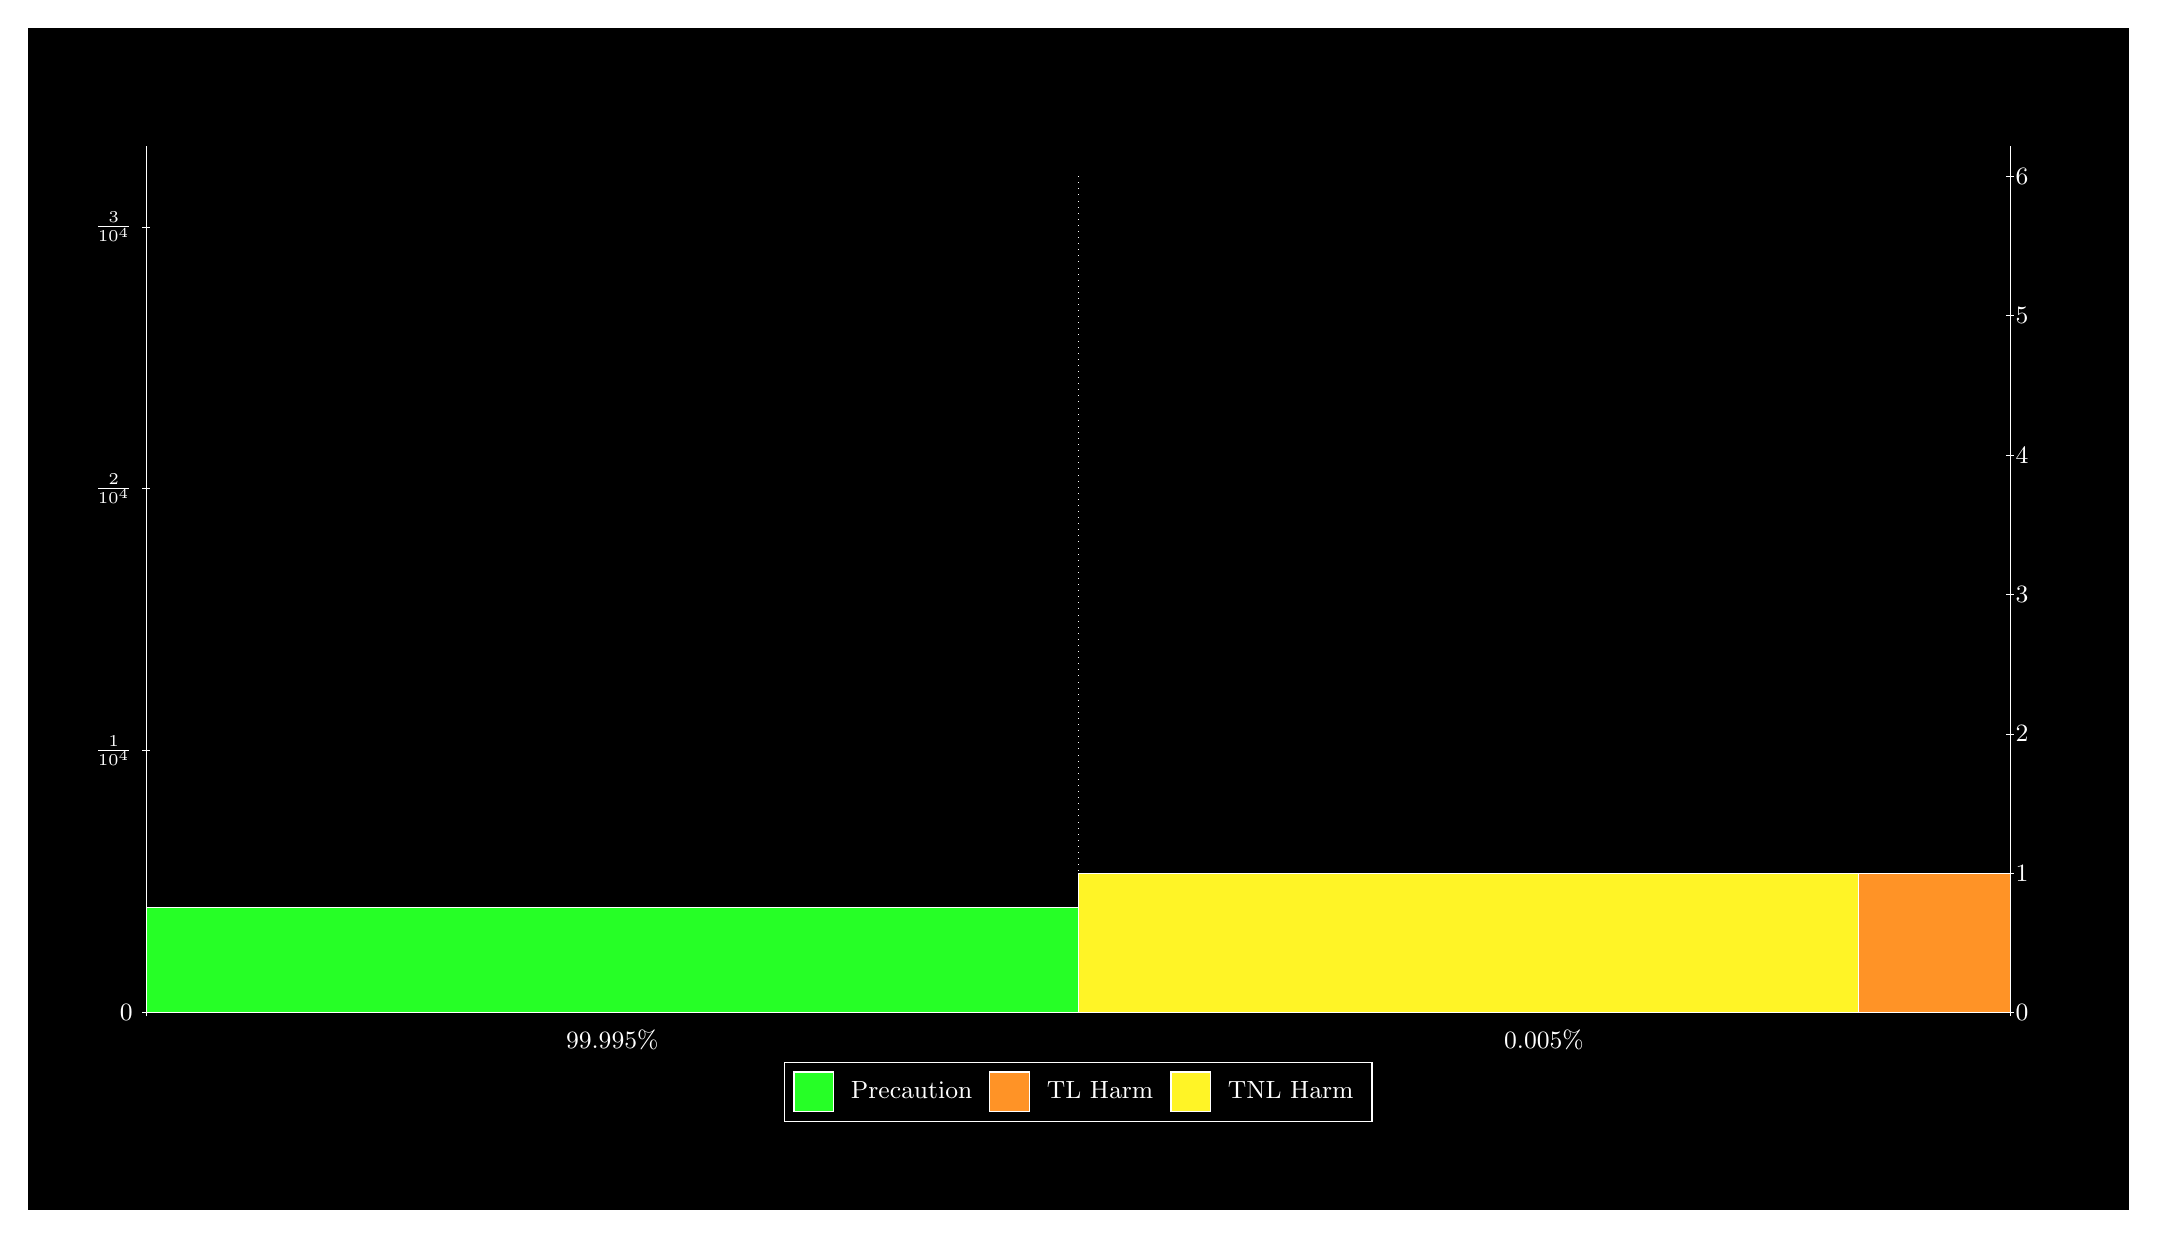
\begin{tikzpicture}
\draw[fill=black] (0,0) rectangle (26.667,15);
\draw[fill=green!85,draw=white,very thin] (1.5,2.5) rectangle (13.333,3.8303);
\draw[fill=green!85,draw=white,very thin] (13.333,2.5) rectangle (23.245,2.5001);
\draw[fill=yellow!85,draw=white,very thin] (13.333,2.5001) rectangle (23.245,4.2697);
\draw[fill=green!85,draw=white,very thin] (23.245,2.5) rectangle (25.167,2.5001);
\draw[fill=orange!85,draw=white,very thin] (23.245,2.5001) rectangle (25.167,4.2697);
\draw[white,very thin] (1.5,2.5) -- (1.5,13.5);
\draw[white,very thin] (1.45,2.5) -- (1.55,2.5);
\node[font=\small,text=white, anchor=east] at (1.45, 2.5) {0};
\draw[white,very thin] (1.45,5.8259) -- (1.55,5.8259);
\node[font=\small,text=white, anchor=east] at (1.45, 5.8259) {$\frac{1}{10^{4}}$};
\draw[white,very thin] (1.45,9.1517) -- (1.55,9.1517);
\node[font=\small,text=white, anchor=east] at (1.45, 9.1517) {$\frac{2}{10^{4}}$};
\draw[white,very thin] (1.45,12.478) -- (1.55,12.478);
\node[font=\small,text=white, anchor=east] at (1.45, 12.478) {$\frac{3}{10^{4}}$};

\draw[white,dotted,very thin] (13.333,2.83) -- (13.333,13.17);
\draw[white,very thin] (25.167,2.5) -- (25.167,13.5);
\draw[white,very thin] (25.117,2.5) -- (25.217,2.5);
\node[font=\small,text=white, anchor=west] at (25.117, 2.5) {0};
\draw[white,very thin] (25.117,4.2697) -- (25.217,4.2697);
\node[font=\small,text=white, anchor=west] at (25.117, 4.2697) {1};
\draw[white,very thin] (25.117,6.0393) -- (25.217,6.0393);
\node[font=\small,text=white, anchor=west] at (25.117, 6.0393) {2};
\draw[white,very thin] (25.117,7.809) -- (25.217,7.809);
\node[font=\small,text=white, anchor=west] at (25.117, 7.809) {3};
\draw[white,very thin] (25.117,9.5786) -- (25.217,9.5786);
\node[font=\small,text=white, anchor=west] at (25.117, 9.5786) {4};
\draw[white,very thin] (25.117,11.348) -- (25.217,11.348);
\node[font=\small,text=white, anchor=west] at (25.117, 11.348) {5};
\draw[white,very thin] (25.117,13.118) -- (25.217,13.118);
\node[font=\small,text=white, anchor=west] at (25.117, 13.118) {6};

\draw[white,very thin] (1.5,2.5) -- (25.167,2.5);
\draw[white,very thin] (1.5,2.45) -- (1.5,2.55);
\node[font=\small,text=white, anchor=north] at (1.5, 2.45) {};
\draw[white,very thin] (25.167,2.45) -- (25.167,2.55);
\node[font=\small,text=white, anchor=north] at (25.167, 2.45) {};

\node[font=\small,text=white,anchor=south] at (7.4167, 1.9) {99.995\%};
\node[font=\small,text=white,anchor=south] at (19.25, 1.9) {0.005\%};
\draw (13.3333,2.5) node (B) {};
\begin{scope}[align=center]
\matrix[scale=0.5,draw=white,below=0.5cm of B,nodes={draw},column sep=0.1cm]{
\node[rectangle,draw,minimum width=0.5cm,minimum height=0.5cm,fill=green!85]{}; & \node[draw=none,font=\small,text=white]{Precaution}; &
\node[rectangle,draw,minimum width=0.5cm,minimum height=0.5cm,fill=orange!85]{}; & \node[draw=none,font=\small,text=white]{TL Harm}; &
\node[rectangle,draw,minimum width=0.5cm,minimum height=0.5cm,fill=yellow!85]{}; & \node[draw=none,font=\small,text=white]{TNL Harm}; \\\\
};\end{scope}

\end{tikzpicture}
\end{document}